\chapter{Analisis}
\label{chap:analisis}

Pada bab ini akan dijelaskan mengenai analisis dari penggunaan \textit{Microsoft Graph API} untuk mendapatkan data \textit{event} yang sudah tercatat di dalam \textit{Outlook Calendar web} dan juga penggunaan dari \textit{Slack API} untuk memampukan program mengubah status yang terdapat pada aplikasi \textit{Slack}, serta analisis dari penggunaan \textit{cron} yang akan digunakan untuk menjalankan program yang disusun secara berkala. Untuk bisa menjalankan program ini, maka dibutuhkan input dari pengguna berupa \textit{login} ke \textit{Windows Live} dan juga memberikan akses kepada program ini untuk mengambil \textit{access token} dan \textit{refresh token} yang akan digunakan untuk mengambil data \textit{event} yang sudah tercatat di dalam \textit{Outlook Calendar}. Selain ke \textit{Windows Live}, program ini juga memerlukan pengguna untuk \textit{login} ke akun yang terdapat di suatu \textit{workspace} di platform \textit{Slack} serta memberikan akses untuk aplikasi ini sebagai aplikasi yang terdaftar dalam \textit{workspace}-nya.  

\section{Analisis Microsoft Graph API}
\label{sec:analisis_microsoft_graph_api}

Pada analisis bagian ini, dilakukan analisis mengenai API yang telah disediakan oleh Microsoft Graph API yang akan digunakan untuk mengambil data acara / event yang dibutuhkan oleh perangkat lunak yang akan dibangun. Akan ada beberapa langkah yang harus dijalankan untuk berhasil mencapai tujuan dari perangkat lunak ini. Analisis dari setiap langkah akan dijelaskan pada subbab \ref{analisis_authorization_code} sampai subbab \ref{analisis_menggunakan_refresh_token}.

\subsection{Analisis Mendapatkan Authorization Code}
\label{analisis_authorization_code}
Untuk mendapatkan authorization code, diperlukan untuk mendaftarkan aplikasi yang akan dibuat ke \textit{Microsoft App Registration Portal}\footnote{https://apps.dev.microsoft.com/}. Dari mendaftarkan aplikasi yang akan dibuat di portal registrasi tersebut akan menghasilkan Application ID, Application Secret, dan juga redirect URL yang akan digunakan. Jika platform yang dipilih adalah web, maka redirect URL harus ditentukan sendiri. Dalam meminta authorization code, aplikasi yang dibuat harus mengirimkan \textit{get request} terlebih dahulu ke \textit{endpoint /authorize} yang membutuhkan parameter seperti yang dijelaskan di tabel \ref{tab:parameter_authorization_code}. 

\begin{table}[H]
	\centering 
	\caption{Tabel parameter \textit{Authorization Code}}
	\label{tab:parameter_authorization_code}
	\begin{tabular}{|p{3cm}|p{3cm}|p{9cm}|}
	\toprule
	\textbf{Parameter} & & \textbf{Deskripsi}\\ \hline 
	\textit{tenant} & wajib & Nilai \textit{tenant} berfungsi untuk mengontrol siapa yang dapat masuk ke dalam aplikasi. Bisa diisi dengan \textit{tenant ID} atau nama domain dari akun \textit{Microsoft}.\\ \hline 
	\textit{client\_id} & wajib & Nilai yang dipakai adalah nilai dari \textit{application ID} yang didapatkan saat mendaftarkan aplikasi di \textit{Microsoft App Registration Portal}.\\ \hline 
	\textit{response\_type} & wajib & Tipe balikan yang diterima dari \textit{request}. Bernilai 				\textit{code} yang berarti akan mengembalikan \textit{code}. \\ \hline 
	\textit{redirect\_uri} & direkomendasikan & \textit{Redirect uri} dari aplikasi yang didaftarkan dimana hasil dari \textit{request} yang didapat akan dikembalikan ke url yang sudah didaftarkan. \\ \hline 
	\textit{scope} & wajib & Daftar izin dari \textit{Microsoft Graph} yang dipisahkan oleh cakupan yang diinginkan dan disetujui oleh pengguna. \\ \hline 
\textit{response\_mode} & direkomendasikan & Menentukan metode yang harus digunakan untuk mengirimkan token yang dihasilkan kembali ke aplikasi. Dapat bernilai \textit{query} atau \textit{form\_post}. \\ \hline 
	\textit{state} & direkomendasikan & Nilai yang diisi saat mengirimkan \textit{request} dan akan dikembalikan juga saat menerima \textit{response}. Tujuan dari nilai ini adalah untuk mencegah pemalsuan permintaan lintas situs. Digunakan untuk menyandikan informasi sebelum \textit{request} untuk otentikasi. Biasanya nilai ini berisi nilai unik secara acak. \\ \bottomrule
\end{tabular}  
\end{table}

Pada parameter scope, dapat diisi dengan nilai offline\_access yang akan menjadikan aplikasi mendapatkan response berupa refresh token yang berguna untuk mendapatkan access token yang baru saat yang lama sudah kadaluarsa. Contoh request yang dikirimkan akan seperti yang terdapat pada contoh table \ref{tab:contoh_request_authorization_code}.

\begin{table}[H]
	\centering 
	\caption{Tabel contoh \textit{request} \textit{Authorization Code}}
	\label{tab:contoh_request_authorization_code}
	\begin{tabular}{|p{12cm}|}
	\toprule
	https://login.microsoftonline.com/\{tenant\}/oauth2/v2.0/authorize?\\
client\_id=6731de76-14a6-49ae-97bc-6eba6914391e\\
\&response\_type=code\\
\&redirect\_uri=http\%3A\%2F\%2Flocalhost\%2Fmyapp\%2F\\
\&response\_mode=query\\
\&scope=offline\_access\%20user.read\%20mail.read\\
\&state=12345\\
	\bottomrule
\end{tabular}  
\end{table}

Dari \textit{request} seperti contoh table \ref{tab:contoh_request_authorization_code}, akan menghasilkan contoh \textit{response} seperti yang terdapat pada table \ref{tab:contoh_response_authorization_code} dengan keterangan parameter seperti yang terdapat pada table \ref{tab:parameter_response_authorization_code}. 

\begin{table}[H]
	\centering 
	\caption{Tabel contoh \textit{response} \textit{Authorization Code}}
	\label{tab:contoh_response_authorization_code}
	\begin{tabular}{|p{9cm}|}
	\toprule
	GET https://localhost/myapp/?\\
code=M0ab92efe-b6fd-df08-87dc-2c6500a7f84d\\
\&state=12345 \\
	\bottomrule
\end{tabular}  
\end{table}

\begin{table}[H]
	\centering 
	\caption{Tabel parameter \textit{response} \textit{Authorization Code}}
	\label{tab:parameter_response_authorization_code}
	\begin{tabular}{|p{3cm}|p{9cm}|}
	\toprule
	\textbf{Parameter} & \textbf{Deskripsi}\\ \hline 
	\textit{code} & Nilai ini merupakan \textit{authorization\_code} yang telah di\textit{request} oleh aplikasi. \textit{Authorization\_code} ini digunakan untuk meminta \textit{access token}. \textit{Authorization code} memiliki waktu kadaluarsa yang singkat yaitu biasanya akan kadaluarsa setelah 10 menit. \\ \hline 
	\textit{state} & Jika saat melakukan \textit{request}, parameter \textit{state} diisi, maka pada saat mengeluarkan \textit{response}, akan mengeluarkan nilai \textit{state} yang sama seperti yang sudah diisi saat melakukan \textit{request}. Aplikasi harus mengidentifikasi apakah nilai \textit{state} saat melakukan \textit{request} dengan nilai \textit{state} di \textit{response} sama atau tidak. \\ \bottomrule
\end{tabular}  
\end{table}

Hasil \textit{response} yang ditampilkan oleh table \ref{tab:contoh_response_authorization_code} muncul karena pada saat \textit{request} di table \ref{tab:contoh_request_authorization_code} terdapat parameter \textit{response\_mode} yang diisi dengan nilai \textit{query} sehingga \textit{response} yang dikembalikan dalam bentuk \textit{query string} dari \textit{redirect url}. 

\subsection{Analisis Mendapatkan Access Token}
\label{analisis_access_token}

Setelah mendapatkan authorization code, langkah selanjutnya yang harus dijalankan sebelum bisa memanggil method API yang dibutuhkan adalah dengan mendapatkan access token. Yang diperlukan untuk bisa mendapatkan access token, maka aplikasi yang dibuat membutuhkan authorization code yang diterima di langkah sebelumnya dan mengirimkan post request kepada endpoint /token. 

Untuk mengirimkan post request, diperlukan request body yang memiliki elemen-elemen seperti yang terdapat di contoh table \ref{tab:contoh_request_access_token}. Adapun penjelasan dari setiap parameter yang terdapat di dalam request body dijelaskan pada table \ref{tab:parameter_request_access_token}. 

\begin{table}[H]
	\centering 
	\caption{Tabel contoh \textit{request} \textit{Access Token}}
	\label{tab:contoh_request_access_token}
	\begin{tabular}{|p{12cm}|}
	\toprule
	POST /common/oauth2/v2.0/token HTTP/1.1\\
Host: https://login.microsoftonline.com\\
Content-Type: application/x-www-form-urlencoded\\
\\
client\_id=6731de76-14a6-49ae-97bc-6eba6914391e\\
\&scope=user.read\%20mail.read\\
\&code=OAAABAAAAiL9Kn2Z27UubvWFPbm0gLWQ\\
JVzCTE9UkP3pSx1aXxUjq3n8b2JRLk4OxVXr...\\
\&redirect\_uri=http\%3A\%2F\%2Flocalhost\%2Fmyapp\%2F\\
\&grant\_type=authorization\_code\\
\&client\_secret=JqQX2PNo9bpM0uEihUPzyrh \\ 
	\bottomrule
	\end{tabular}  
\end{table}

\begin{table}[H]
	\centering 
	\caption{Tabel parameter \textit{request} \textit{Access Token}}
	\label{tab:parameter_request_access_token}
	\begin{tabular}{|p{3cm}|p{3cm}|p{9cm}|}
	\toprule
	 \textbf{Parameter} & & \textbf{Deskripsi}\\ \hline 
	\textit{tenant} & wajib & Nilai \textit{tenant} berfungsi untuk mengontrol siapa yang dapat masuk ke dalam aplikasi. Bisa diisi dengan \textit{tenant ID} atau nama domain dari akun \textit{Microsoft}.\\ \hline 
	\textit{client\_id} & wajib & Nilai yang dipakai adalah nilai dari \textit{application ID} yang didapatkan saat mendaftarkan aplikasi di \textit{Microsoft App Registration Portal}.\\ \hline 
	\textit{grant\_type} & wajib & Harus diisi dengan nilai authorization\_code untuk alur authorization code. \\ \hline
	\textit{scope} & wajib & Daftar izin dari \textit{Microsoft Graph} yang dipisahkan oleh cakupan yang diinginkan dan disetujui oleh pengguna. Dalam langkah ini, nilai dari scope pada langkah sebelumnya harus sama dengan langkah ini.  \\ \hline 
	\textit{code} & wajib & Authorization code yang didapat dari langkah sebelumnya. \\ \hline  
	\textit{redirect\_uri} & wajib & \textit{Redirect uri} yang sama yang dipakai untuk mendapatkan authorization code. \\ \hline 
	\textit{client\_secret} & wajib untuk \textit{web apps} & Application secret yang dibuat saat mendaftarkan aplikasi di portal registrasi untuk aplikasi yang didaftarkan.\\
	\bottomrule
	\end{tabular}  
\end{table}

Dari contoh request yang dilakukan pada table\ref{tab:contoh_request_access_token}, maka akan dihasilkan contoh token seperti pada table \ref{tab:contoh_response_access_token} yang memiliki keterangan dari hasil yang dikembalikan pada table\ref{tab:parameter_response_access_token}. 

\begin{table}[H]
	\centering 
	\caption{Tabel contoh \textit{response} \textit{Access Token}}
	\label{tab:contoh_response_access_token}
	\begin{tabular}{|p{9cm}|}
	\toprule
	\{\\
    "token\_type": "Bearer",\\
    "scope": "user.read\%20Fmail.read",\\
    "expires\_in": 3600,\\
    "access\_token": "eyJ0eXAiOiJKV1QiLCJhbG\\
    ciOiJSUzI1NiIsIng1dCI6Ik5HVEZ2ZEstZnl0aEV1Q...",\\
    "refresh\_token": "AwABAAAAvPM1KaPlrEqdF\\
    SBzjqfTGAMxZGUTdM0t4B4..."\\
	\}\\ 
	\bottomrule
	\end{tabular}  
\end{table}

\begin{table}[H]
	\centering 
	\caption{Tabel parameter \textit{response} \textit{Access Token}}
	\label{tab:parameter_response_access_token}
	\begin{tabular}{|p{3cm}|p{9cm}|}
	\toprule
	 \textbf{Parameter} & \textbf{Deskripsi}\\ \hline 
	\textit{token\_type} & Menunjukkan nilai dari token. Satu-satunya jenis token yang didukung oleh Azure AD adalah Bearer.\\ \hline 
	\textit{scope} & Nilai scope yang valid untuk access\_token yang diberikan.  \\ \hline 
	\textit{expires\_in} & Lamanya access token akan berlaku(dalam detik). \\ \hline  
	\textit{access\_token} & Access token yang diminta. Dengan memakai ini, maka aplikasi bisa memanggil Microsoft Graph. \\ \hline 
	\textit{refresh\_token} & Refresh token ini berguna untuk meminta kembali access token setelah access token itu berakhir. Refresh token memiliki umur yang panjang dan dapat digunakan untuk mempertahankan akses ke source. \\
	\bottomrule
	\end{tabular}  
\end{table}

\subsection{Analisis Menggunakan Access Token untuk memanggil Microsoft Graph}
\label{analisis_menggunakan_access_token}
Setelah mendapatkan access token, panggilan ke Microsoft Graph pun bisa dilakukan dengan syarat menyertakan access token di authorization header di setiap request yang dikirim. Pada table\ref{tab:contoh_request_call_microsoft_graph} menunjukkan contoh request untuk mendapatkan profile dari pengguna yang masuk. 

\begin{table}[H]
	\centering 
	\caption{Tabel contoh \textit{request} \textit{call Microsoft Graph}}
	\label{tab:contoh_request_call_microsoft_graph}
	\begin{tabular}{|p{9cm}|}
	\toprule
	GET https://graph.microsoft.com/v1.0/me \\
Authorization: Bearer eyJ0eXAiO ... 0X2tnSQLEANnSPHY0gKcgw\\
Host: graph.microsoft.com \\
	\bottomrule
	\end{tabular}  
\end{table}

Jika request yang dikirimkan berhasil, maka akan mendapatkan response yang akan terlihat mirip dengan contoh seperti pada table \ref{tab:contoh_response_call_microsoft_graph}

\begin{table}[H]
	\centering 
	\caption{Tabel contoh \textit{response} \textit{call Microsoft Graph}}
	\label{tab:contoh_response_call_microsoft_graph}
	\begin{tabular}{|p{12cm}|}
	\toprule
	HTTP/1.1 200 OK\\
Content-Type: application/json;\\
odata.metadata=minimal;\\
odata.streaming=true;\\
IEEE754Compatible=false;\\
charset=utf-8\\
\\
request-id: f45d08c0-6901-473a-90f5-7867287de97f\\
client-request-id: f45d08c0-6901-473a-90f5-7867287de97f\\
OData-Version: 4.0\\
Duration: 727.0022\\
Date: Thu, 20 Apr 2017 05:21:18 GMT\\
Content-Length: 407\\
\\
\{\\
    "@odata.context":"https://graph.microsoft.com/v1.0/\\
    $metadata\#users/$entity",\\
    "id":"12345678-73a6-4952-a53a-e9916737ff7f",\\
    "businessPhones":[\\
        "+1 555555555"\\
    ],\\
    "displayName":"Chris Green",\\
    "givenName":"Chris",\\
    "jobTitle":"Software Engineer",\\
    "mail":null,\\
    "mobilePhone":"+1 5555555555",\\
    "officeLocation":"Seattle Office",\\
    "preferredLanguage":null,\\
    "surname":"Green",\\
    "userPrincipalName":"ChrisG@contoso.onmicrosoft.com"\\
\}\\
	\bottomrule
	\end{tabular}  
\end{table}

\subsection{Analisis Menggunakan Refresh Token untuk Mendapatkan Access Token Baru}
\label{analisis_menggunakan_refresh_token}
Access token memiliki waktu yang singkat dan ketika sudah kadaluarsa, maka aplikasi yang akan dibuat harus meminta kembali access token yang supaya bisa terus mengakses data yang ada di dalam Microsoft Graph. Cara mendapatkan access token yang baru dengan menggunakan refresh token adalah dengan cara mengirimkan post request sekali lagi kepada endpoint /token dan untuk kali ini, gunakan refresh token sebagai parameter yang dikirimkan dan juga grant type yang berisikan refresh token dalam body dari request yang dilakukan seperti contoh pada table \ref{tab:contoh_request_refresh_token} dengan keterangan parameter seperti yang dijelaskan pada table \ref{tab:parameter_request_refresh_token}. 

\begin{table}[H]
	\centering 
	\caption{Tabel contoh \textit{request} menggunakan \textit{Refresh Token}}
	\label{tab:contoh_request_refresh_token}
	\begin{tabular}{|p{12cm}|}
	\toprule
	POST /common/oauth2/v2.0/token HTTP/1.1\\
Host: https://login.microsoftonline.com\\
Content-Type: application/x-www-form-urlencoded\\
\\
client\_id=6731de76-14a6-49ae-97bc-6eba6914391e\\
\&scope=user.read\%20mail.read\\
\&refresh\_token=OAAABAAAAiL9Kn2Z27UubvWFPbm0gLWQJVzCTE\\
9UkP3pSx1aXxUjq...\\
\&redirect\_uri=http\%3A\%2F\%2Flocalhost\%2Fmyapp\%2F\\
\&grant\_type=refresh\_token\\
\&client\_secret=JqQX2PNo9bpM0uEihUPzyrh\\
	\bottomrule
	\end{tabular}  
\end{table}

\begin{table}[H]
	\centering 
	\caption{Tabel parameter \textit{request} \textit{Refresh Token}}
	\label{tab:parameter_request_refresh_token}
	\begin{tabular}{|p{3cm}|p{3cm}|p{9cm}|}
	\toprule
	 \textbf{Parameter} & & \textbf{Deskripsi}\\ \hline 
	\textit{client\_id} & wajib & Nilai yang dipakai adalah nilai dari \textit{application ID} yang didapatkan saat mendaftarkan aplikasi di \textit{Microsoft App Registration Portal}.\\ \hline 
	\textit{grant\_type} & wajib & Harus diisi dengan nilai refresh\_token. \\ \hline
	\textit{scope} & wajib & Daftar izin dari \textit{Microsoft Graph} yang dipisahkan oleh cakupan yang diinginkan dan disetujui oleh pengguna. Dalam langkah ini, nilai dari scope pada langkah meminta authorization\_code harus sama dengan langkah ini.  \\ \hline 
	\textit{refresh\_token} & wajib & Refresh token yang didapat saat merequest token yang pertama kali. \\ \hline  
	\textit{redirect\_uri} & wajib & \textit{Redirect uri} yang sama yang dipakai untuk mendapatkan authorization code. \\ \hline 
	\textit{client\_secret} & wajib untuk \textit{web apps} & Application secret yang dibuat saat mendaftarkan aplikasi di portal registrasi untuk aplikasi yang didaftarkan.\\
	\bottomrule
	\end{tabular}  
\end{table}

Jika request ini berhasil, maka akan mengembalikan response seperti pada table \ref{tab:contoh_response_refresh_token} yang memiliki keterangan parameter yang dikembalikannya seperti pada table \ref{tab:parameter_response_refresh_token}. 
\\
\begin{table}[H]
	\centering 
	\caption{Tabel contoh \textit{response} menggunakan \textit{Refresh Token}}
	\label{tab:contoh_response_refresh_token}
	\begin{tabular}{|p{12cm}|}
	\toprule
	\{\\
    "access\_token": "eyJ0eXAiOiJKV1QiLCJhbGciOiJSUzI1NiI\\
    sIng1dCI6Ik5HVEZ2ZEstZnl0aEV1Q...",\\
    "token\_type": "Bearer",\\
    "expires\_in": 3599,\\
    "scope": "user.read\%20mail.read",\\
    "refresh\_token": "AwABAAAAvPM1KaPlrEqdFSBzjq\\
    fTGAMxZGUTdM0t4B4...",\\
\}\\
	\bottomrule
	\end{tabular}  
\end{table}

\begin{table}[H]
	\centering 
	\caption{Tabel parameter \textit{response} \textit{Refresh Token}}
	\label{tab:parameter_response_refresh_token}
	\begin{tabular}{|p{3cm}|p{9cm}|}
	\toprule
	 \textbf{Parameter} & \textbf{Deskripsi}\\ \hline 
	 \textit{access\_token} & Access token yang diminta. Dengan memakai ini, maka aplikasi bisa memanggil Microsoft Graph. \\ \hline 
	\textit{token\_type} & Menunjukkan nilai dari token. Satu-satunya jenis token yang didukung oleh Azure AD adalah Bearer.\\ \hline 
	\textit{expires\_in} & Lamanya access token akan berlaku(dalam detik). \\ \hline 
	\textit{scope} & Nilai scope yang valid untuk access\_token yang diberikan.  \\ \hline  
	\textit{refresh\_token} & Refresh token ini berguna untuk meminta kembali access token setelah access token itu berakhir. Refresh token memiliki umur yang panjang dan dapat digunakan untuk mempertahankan akses ke source. \\
	\bottomrule
	\end{tabular}  
\end{table}

\subsection{Analisis Mendapatkan Data Events}
\label{sec:analisis_mendapatkan_data_events}
Data event di dalam Microsoft Graph tersimpan di dalam objek event yang memiliki relasi dengan objek user dari pengguna. Untuk dapat mengakses event yang memiliki relasi dengan user, aplikasi yang akan dibuat harus menjalankan method yang dimiliki objek user yaitu method list events mengirimkan get request kepada endpoint /me/events. List events sendiri adalah method yang berfungsi untuk mengembalikan objek-objek event yang berkaitan dengan objek user pengguna. Untuk setiap operasi get yang mengembalikan objek event di Microsoft Graph, ada sebuah parameter header ``Prefer:outlook.timezone'' yang berfungsi untuk menentukan time zone untuk mulainya dan berakhirnya event. Sebagai contoh, dapat dilihat pada table \ref{tab:contoh_header_time_zone}. 

\begin{table}[H]
	\centering 
	\caption{Tabel contoh \textit{header time zone}}
	\label{tab:contoh_header_time_zone}
	\begin{tabular}{|p{9cm}|}
	\toprule
	 Prefer: outlook.timezone="Eastern Standard Time" \\
	\bottomrule
	\end{tabular}  
\end{table}

Pada table \ref{tab:contoh_header_time_zone}, outlook timezone diatur menjadi Eastern Standard Time yang nantinya semua event yang dipanggil dengan header seperti itu akan mengembalikan starttime dan endtime dari event akan disesuaikan dengan zona waktu Eastern Standard Time. 

Untuk bisa mengakses method ini, maka diperlukan format header dari request seperti yang akan dijelaskan pada table \ref{tab:parameter_header_time_zone}. 

\begin{table}[H]
	\centering 
	\caption{Tabel parameter \textit{header time zone}}
	\label{tab:parameter_header_time_zone}
	\begin{tabular}{|p{3cm}|p{3cm}|p{9cm}|}
	\toprule
	 \textbf{Nama} & \textbf{\textit{Type}} & \textbf{Deskripsi}\\ \hline
	 \textit{Authorization} & \textit{String} & Bearer {token}. Bersifat wajib diisi. \\ \hline
	 \textit{Prefer:}& & \\
	 \textit{outlook.timezone} & \textit{String} & Digunakan untuk menentukan zona waktu yang akan dipakai untuk data yang akan dikembalikan. Bersifat optional. \\ \hline
	 \textit{Prefer:}& & \\
	 \textit{outlook.body-content-type} & \textit{String} & Merupakan nilai yang mengatur properti dari response body yang akan dikembalikan. Nilai bisa berupa ``text'' atau ``html''. Nilai default dari parameter ini adalah html. Bersifat optional. \\ \hline
	\bottomrule
	\end{tabular}  
\end{table}

Request ini juga bisa menerima parameter \$select yang berbentuk string query sebagai filter mengenai field apa saja yang mau diambil dari objek event. Dapat dilihat fungsi dari parameter string query \$select seperti pada contoh table \ref{tab:contoh_request_event} dan contoh responsenya pada table \ref{tab:contoh_response_event}. 

\begin{table}[H]
	\centering 
	\caption{Tabel contoh \textit{request event}}
	\label{tab:contoh_request_event}
	\begin{tabular}{|p{12cm}|}
	\toprule
	GET https://graph.microsoft.com/v1.0/me/events?\\
	\$select=subject,bodyPreview,organizer,start,end,location\\
	Prefer: outlook.timezone="Pacific Standard Time"\\
	\bottomrule
	\end{tabular}  
\end{table}

\begin{table}[H]
	\centering 
	\caption{Tabel contoh \textit{response event}}
	\label{tab:contoh_response_event}
	\begin{tabular}{|p{15cm}|}
	\toprule
	\begin{lstlisting}
{
    "@odata.context":"https://graph.microsoft.com/v1.0/$metadata
    #users('cd209b0b-3f83-4c35-82d2-d88a61820480')/events(subject
    ,bodyPreview,organizer,start,end,location)",
    "value":[
        {
            "@odata.etag":"W/\"ZlnW4RIAV06KYYwlrfNZvQAAKGWwbw==\"",
            "id":"AAMkAGIAAAoZDOFAAA=",
            "subject":"Orientation ",
            "bodyPreview":"Dana, this is the time you selected for 
            our orientation. Please bring the notes I sent you.",
            "start":{
                "dateTime":"2017-04-21T10:00:00.0000000",
                "timeZone":"Pacific Standard Time"
            },"end":{
                "dateTime":"2017-04-21T12:00:00.0000000",
                "timeZone":"Pacific Standard Time"
            },"location": {
                "displayName": "Assembly Hall",
                "locationType": "default",
                "uniqueId": "Assembly Hall",
                "uniqueIdType": "private"
            },"locations": [{
                    "displayName": "Assembly Hall",
                    "locationType": "default",
                    "uniqueIdType": "unknown"
            }],                
            "organizer":{
                "emailAddress":{
                    "name":"Samantha Booth",
                    "address":"samanthab@a830edad905084922E170
                    20313.onmicrosoft.com"
                }
            }
        }
    ]
}
\end{lstlisting}\\
	\bottomrule
	\end{tabular}  
\end{table}

\section{Analisis Slack API}
\label{sec:analisis_slack_api}
Untuk dapat memakai dan mengakses \textit{method-method} yang disediakan oleh \textit{Slack}, dibutuhkan mendaftarkan aplikasi yang akan dibuat untuk bisa memperoleh \textit{Client ID} yang nantinya dibutuhkan untuk bisa mendapatkan \textit{authorization code} serta \textit{access token}. Sama seperti di \textit{Microsoft Graph API}, di dalam \textit{Slack API access token} dibutuhkan sebagai otorisasi untuk bisa mengakses \textit{method-method} yang disediakan oleh \textit{Slack}. Jika tidak memiliki \textit{access token}, maka seluruh \textit{method} yang dicoba di\textit{request} tidak akan mengembalikkan hasil dan dianggap sebagai \textit{request} yang tidak \textit{valid}. 

Pada sesi ini akan dibutuhkan \textit{method} dari \textit{Slack API} yang bisa mengubah status yang terdapat pada bagian \textit{user.profile}. Dari informasi yang disediakan oleh Slack secara \textit{online}, bahwa status tergabung dalam \textit{user.profile}, maka untuk memenuhi dari kebutuhan di sisi ini dicoba menggunakan \textit{method-method} yang bisa untuk mengakses kepada objek \textit{user.profile}. Karena di sisi ini akan mengubah nilai dari status, asumsi sementara dari \textit{method} yang bisa dipakai dari sisi ini adalah \textit{method users.profile.set} yang akan berguna untuk mengubah isi dari profil pengguna yang di dalamnya terdapat status. 

\section{Analisis Heroku Scheduler}
\label{sec:analisis_cron}
Untuk menjalankan aplikasi yang akan dibuat untuk mengambil data dari Microsoft Graph yang berhubungan dengan pengambilan data event, maka diperlukan aplikasi yang bisa mengambil data dengan mengirimkan request kepada Microsoft Graph, tetapi pengambilan data dibutuhkan secara berkala untuk memeriksa secara berkala data yang sudah dimasukkan ke dalam Microsoft Graph. Heroku Scheduler merupakan add-ons dari Heroku yang dapat menjalankan perintah secara berkala sesuai dengan yang sudah diatur sejak awal. Untuk menambahan job pada Heroku Scheduler, dapat diakses melalui command line dengan perintah seperti:

\begin{lstlisting}
\$ heroku addons:open scheduler
\end{lstlisting}

Setelah halaman baru pada browser muncul, pilih tombol untuk menambahkan job di scheduler dengan menekan tombol ``Add Job''. Pada Heroku Scheduler tersedia interval untuk menjalankan sebuah job yaitu setiap 10 menit sekali, atau setiap jam pada menit ke, atau setiap hari pada jam ke.

Untuk memperkecil perangkat lunak melewatkan event yang tercatat di Outlook Calendar, maka bagian dari perangkat lunak yang melakukan sinkronisasi akan dijalankan setiap 10 menit sekali. 

\section{Analisis Diagram Alir Sistem}
\subsection{Bagian perangkat lunak yang berinteraksi dengan pengguna}

\begin{figure}[h]
  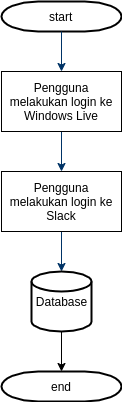
\includegraphics[width=3cm]{./Gambar/workflow.png}
  \centering
  \caption{Diagram alir sistem pada bagian perangkat lunak yang berinteraksi dengan user.}
  \label{fig:workflow1}
\end{figure}

Diagram alir pada gambar \ref{fig:workflow1} menunjukkan aliran proses yang terjadi pada bagian perangkat lunak yang berinteraksi dengan pengguna, berikut penjelasan dari aliran proses tersebut:
\begin{itemize}
    \item Proses pengguna melakukan login ke Windows Live adalah proses dimana perangkat lunak akan mendapatkan access token dari Windows Live dan data lainnya yang dibutuhkan untuk mendapatkan data dari event yang tercatat di dalam Outlook Calendar. 
    \item Proses pengguna melakukan login ke Slack adalah proses dimana perangkat lunak akan mendapatkan access token dari Slack untuk bisa mengganti status jika ada suatu event yang berjalan. 
    \item Setelah kedua proses dijalankan, maka semua data yang dibutuhkan akan dimasukkan ke dalam database agar bisa dijalankan juga dengan bagian dari perangkat lunak yang lain. 
\end{itemize}
\clearpage

\subsection{Bagian perangkat lunak yang dijalankan secara berkala}

\begin{figure}[h]
  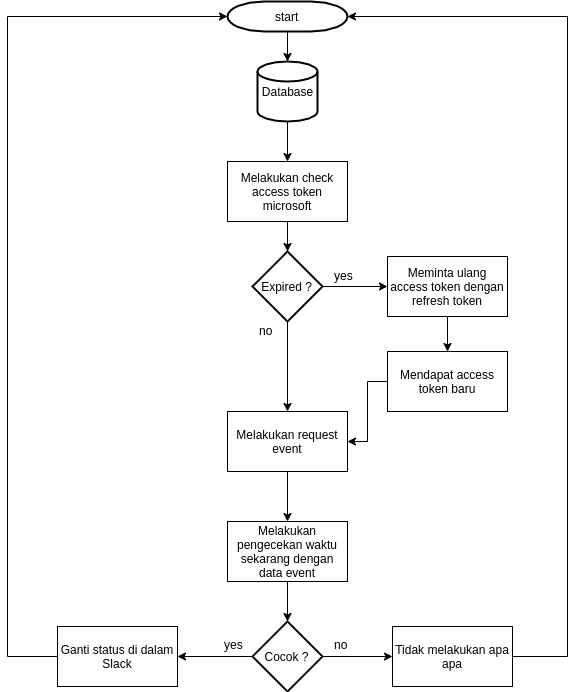
\includegraphics[width=10cm]{./Gambar/workflow2.png}
  \centering
  \caption{Diagram alir sistem pada bagian perangkat lunak yang dijalankan secara berkala.}
  \label{fig:workflow2}
\end{figure}

Diagram alir pada gambar \ref{fig:workflow2} menunjukkan aliran proses yang dilakukan oleh bagian perangkat lunak yang dijalankan secara berkala, berikur penjelasan dari aliran proses tersebut:
\begin{itemize}
    \item Pertama-tama perangkat lunak akan mengambil data dari dalam basis data. 
    \item Lalu terdapat proses untuk melakukan pengecekan untuk access token dari Microsoft dikarenakan access token ini memiliki waktu kadaluarsa. 
    \item Jika access token sudah kadaluarsa, maka meminta ulang access token dengan menggunakan refresh token.
    \item Jika access token belum expired, maka dilanjutkan dengan meminta data mengenai event yang ada di Outlook Calendar. 
    \item Jika setelah melakukan permintaan ulang access token dan sudah mendapatkan access token yang baru, maka meminta data mengenai event yang ada di Outlook Calendar. 
    \item Lalu setelah mendapatkan data event, maka melakukan pengecekan data event dengan waktu sekarang. Jika waktu sekarang beririsan dengan event yang sedang berjalan, maka perangkat lunak akan mengganti status yang ada pada Slack. 
    \item Jika tidak ada yang beririsan, maka tidak akan melakukan apa-apa. 
    \item Proses ini akan berjalan kembali secara berkala sesuai dengan waktu yang sudah diatur di dalam Heroku Scheduler. 
\end{itemize}

\section{Analisis Diagram Use Case}
\begin{figure}[h]
  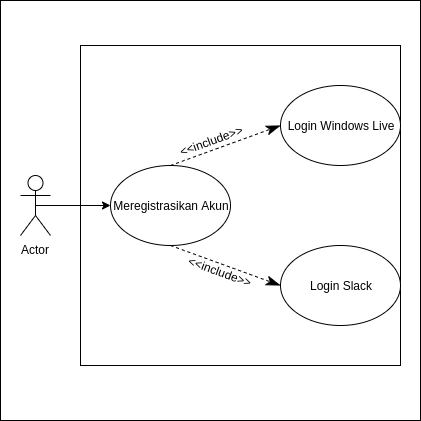
\includegraphics[width=10cm]{./Gambar/usecase.png}
  \centering
  \caption{Diagram Use Case.}
  \label{fig:usecase}
\end{figure}

\begin{itemize}
    \item \textbf{Skenario \textit{Login Windows Live}}\\
    Nama : Login Windows Live\\
    Aktor : Pengguna\\
    Kondisi Awal : Pengguna memiliki akun Windows Live\\
    Deskripsi : Pengguna melakukan login pada aplikasi Windows Live dengan akun pribadinya.\\
    Kondisi Akhir : Pengguna berhasil melakukan login ke Windows Live\\
    Skenario : 
    \begin{itemize}
        \item Pengguna melakukan login dengan id dan kata sandi yang dimilikinya. 
        \item Pengguna mengizinkan akun Windows Live miliknya bekerjasama dengan perangkat lunak ini. 
        \item Pengguna berhasil melakukan login ke Windows Live dan perangkat lunak mendapatkan akses. 
    \end{itemize}
    Eksepsi : 
    \begin{itemize}
        \item Pengguna tidak memiliki akun Windows Live. 
    \end{itemize}
    
    \item \textbf{Skenario \textit{Login Slack}}\\
    Nama : Login Slack\\
    Aktor : Pengguna\\
    Kondisi Awal : Pengguna memiliki akun Slack yang tergabung dalam suatu workspace\\
    Deskripsi : Pengguna melakukan login pada aplikasi Slack di workspace pengguna tergabung.\\
    Kondisi Akhir : Pengguna berhasil melakukan login ke workspace Slack\\
    Skenario : 
    \begin{itemize}
        \item Pengguna melakukan login dengan id dan kata sandi yang dimilikinya. 
        \item Pengguna mengizinkan perangkat lunak ini menjadi bagian di dalam workspace Slack sebagai aplikasi pembantu di workspace tersebut. 
        \item Pengguna berhasil melakukan login ke Slack dan perangkat lunak mendapatkan akses. 
    \end{itemize}
    Eksepsi : 
    \begin{itemize}
        \item Pengguna tidak memiliki akun Slack dan atau tidak terdaftar di dalam workspace manapun. 
    \end{itemize}
    
    \item \textbf{Skenario Meregistrasikan Akun}
    Nama : Meregistrasikan Akun\\
    Aktor : Pengguna\\
    Kondisi Awal : Pengguna memiliki akun Windows Live dan Slack\\
    Deskripsi : Pengguna meregistrasikan akunnya untuk bisa melakukan sinkronisasi antara Outlook Calendar dengan Slack.\\
    Kondisi Akhir : Pengguna berhasil meregistrasikan akunnya\\
    Skenario : 
    \begin{itemize}
        \item Pengguna melakukan login pada Windows Live. 
        \item Pengguna melakukan login pada Slack. 
        \item Pengguna berhasil melakukan login ke kedua aplikasi tersebut dan pengguna berhasil meregistrasikan akunnya untuk disinkronkan. 
    \end{itemize}
    Eksepsi : 
    \begin{itemize}
        \item Pengguna tidak memiliki akun Windows Live dan Slack. 
    \end{itemize}
    
\end{itemize}

\section{Analisis Data Flow Diagram}

\begin{figure}[h]
  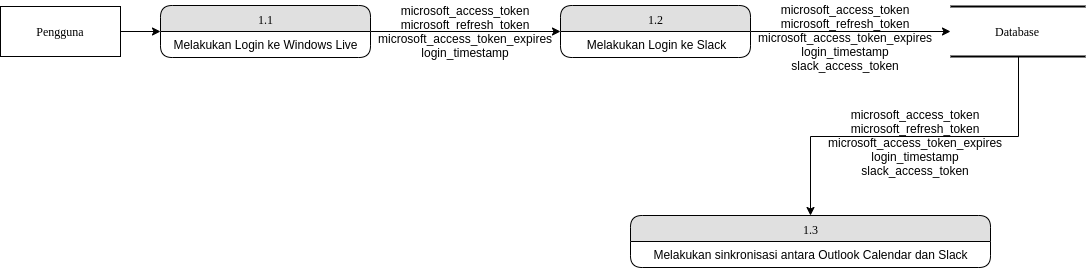
\includegraphics[width=10cm]{./Gambar/DFD.png}
  \centering
  \caption{Data Flow Diagram.}
  \label{fig:dfd}
\end{figure}

Diagram alir data pada gambar \ref{fig:dfd} menunjukkan aliran data pada sistem, nerikut penjelasan dari setiap proses aliran data tersebut:
\begin{itemize}
    \item \textbf{Proses melakukan \textit{login} ke \textit{Windows Live}}\\
    Input : ID dan Password akun Windows Live.\\
    Output : microsoft\_access\_token, microsoft\_access\_token\_expires, microsoft\_refresh\_token, login\_timestamp\\
    Proses ini merupakan proses meminta access token dan segala data yang diperlukan untuk mendapatkan data event dari Outlook Calendar. Proses ini menghasilkan data microsoft\_access\_token, microsoft\_access\_token\_expires, microsoft\_refresh\_token, login\_timestamp. 
    \item \textbf{Proses melakukan \textit{login} ke \textit{Slack}}\\
    Input : \textit{ID} dan \textit{Password} beserta \textit{workspace} di \textit{Slack}.\\
    Output : microsoft\_access\_token, microsoft\_access\_token\_expires, microsoft\_refresh\_token, login\_timestamp, slack\_access\_token\\
    Proses ini merupakan proses meminta access token kepada aplikasi Slack agar perangkat lunak bisa mengubah status di dalam aplikasi Slack. Proses ini menghasilkan data microsoft\_access\_token, microsoft\_access\_token\_expires, microsoft\_refresh\_token, login\_timestamp, slack\_access\_token. 
    \item \textbf{Proses melakukan sinkronisasi antara Outlook Calendar dan Slack}\\
    Input : Data dari basis data seperti token dari Windows Live dan juga dari Slack.\\
    Output : -
    Proses ini merupakan proses sinkronisasi aplikasi Outlook Calendar dan juga Slack dengan cara mengambil data event yang terdapat di Outlook Calendar menggunakan token yang didapat dari Windows Live dan juga menggunakan token yang didapat dari Slack untuk dapat mengubah status dalam Slack jika waktu event dan waktu sekarang beririsan. 
\end{itemize}
